
\documentclass[foo.tex]{subfiles}
\begin{document}
\renewcommand\theequation{\thesection\arabic{equation}}
\renewcommand\thefigure{\thesection\arabic{figure}}
\setcounter{equation}{0}
\setcounter{figure}{0}

\section{The Yield-Outflow Degeneracy}
\label{sec:degeneracy}

\begin{figure*}
\centering
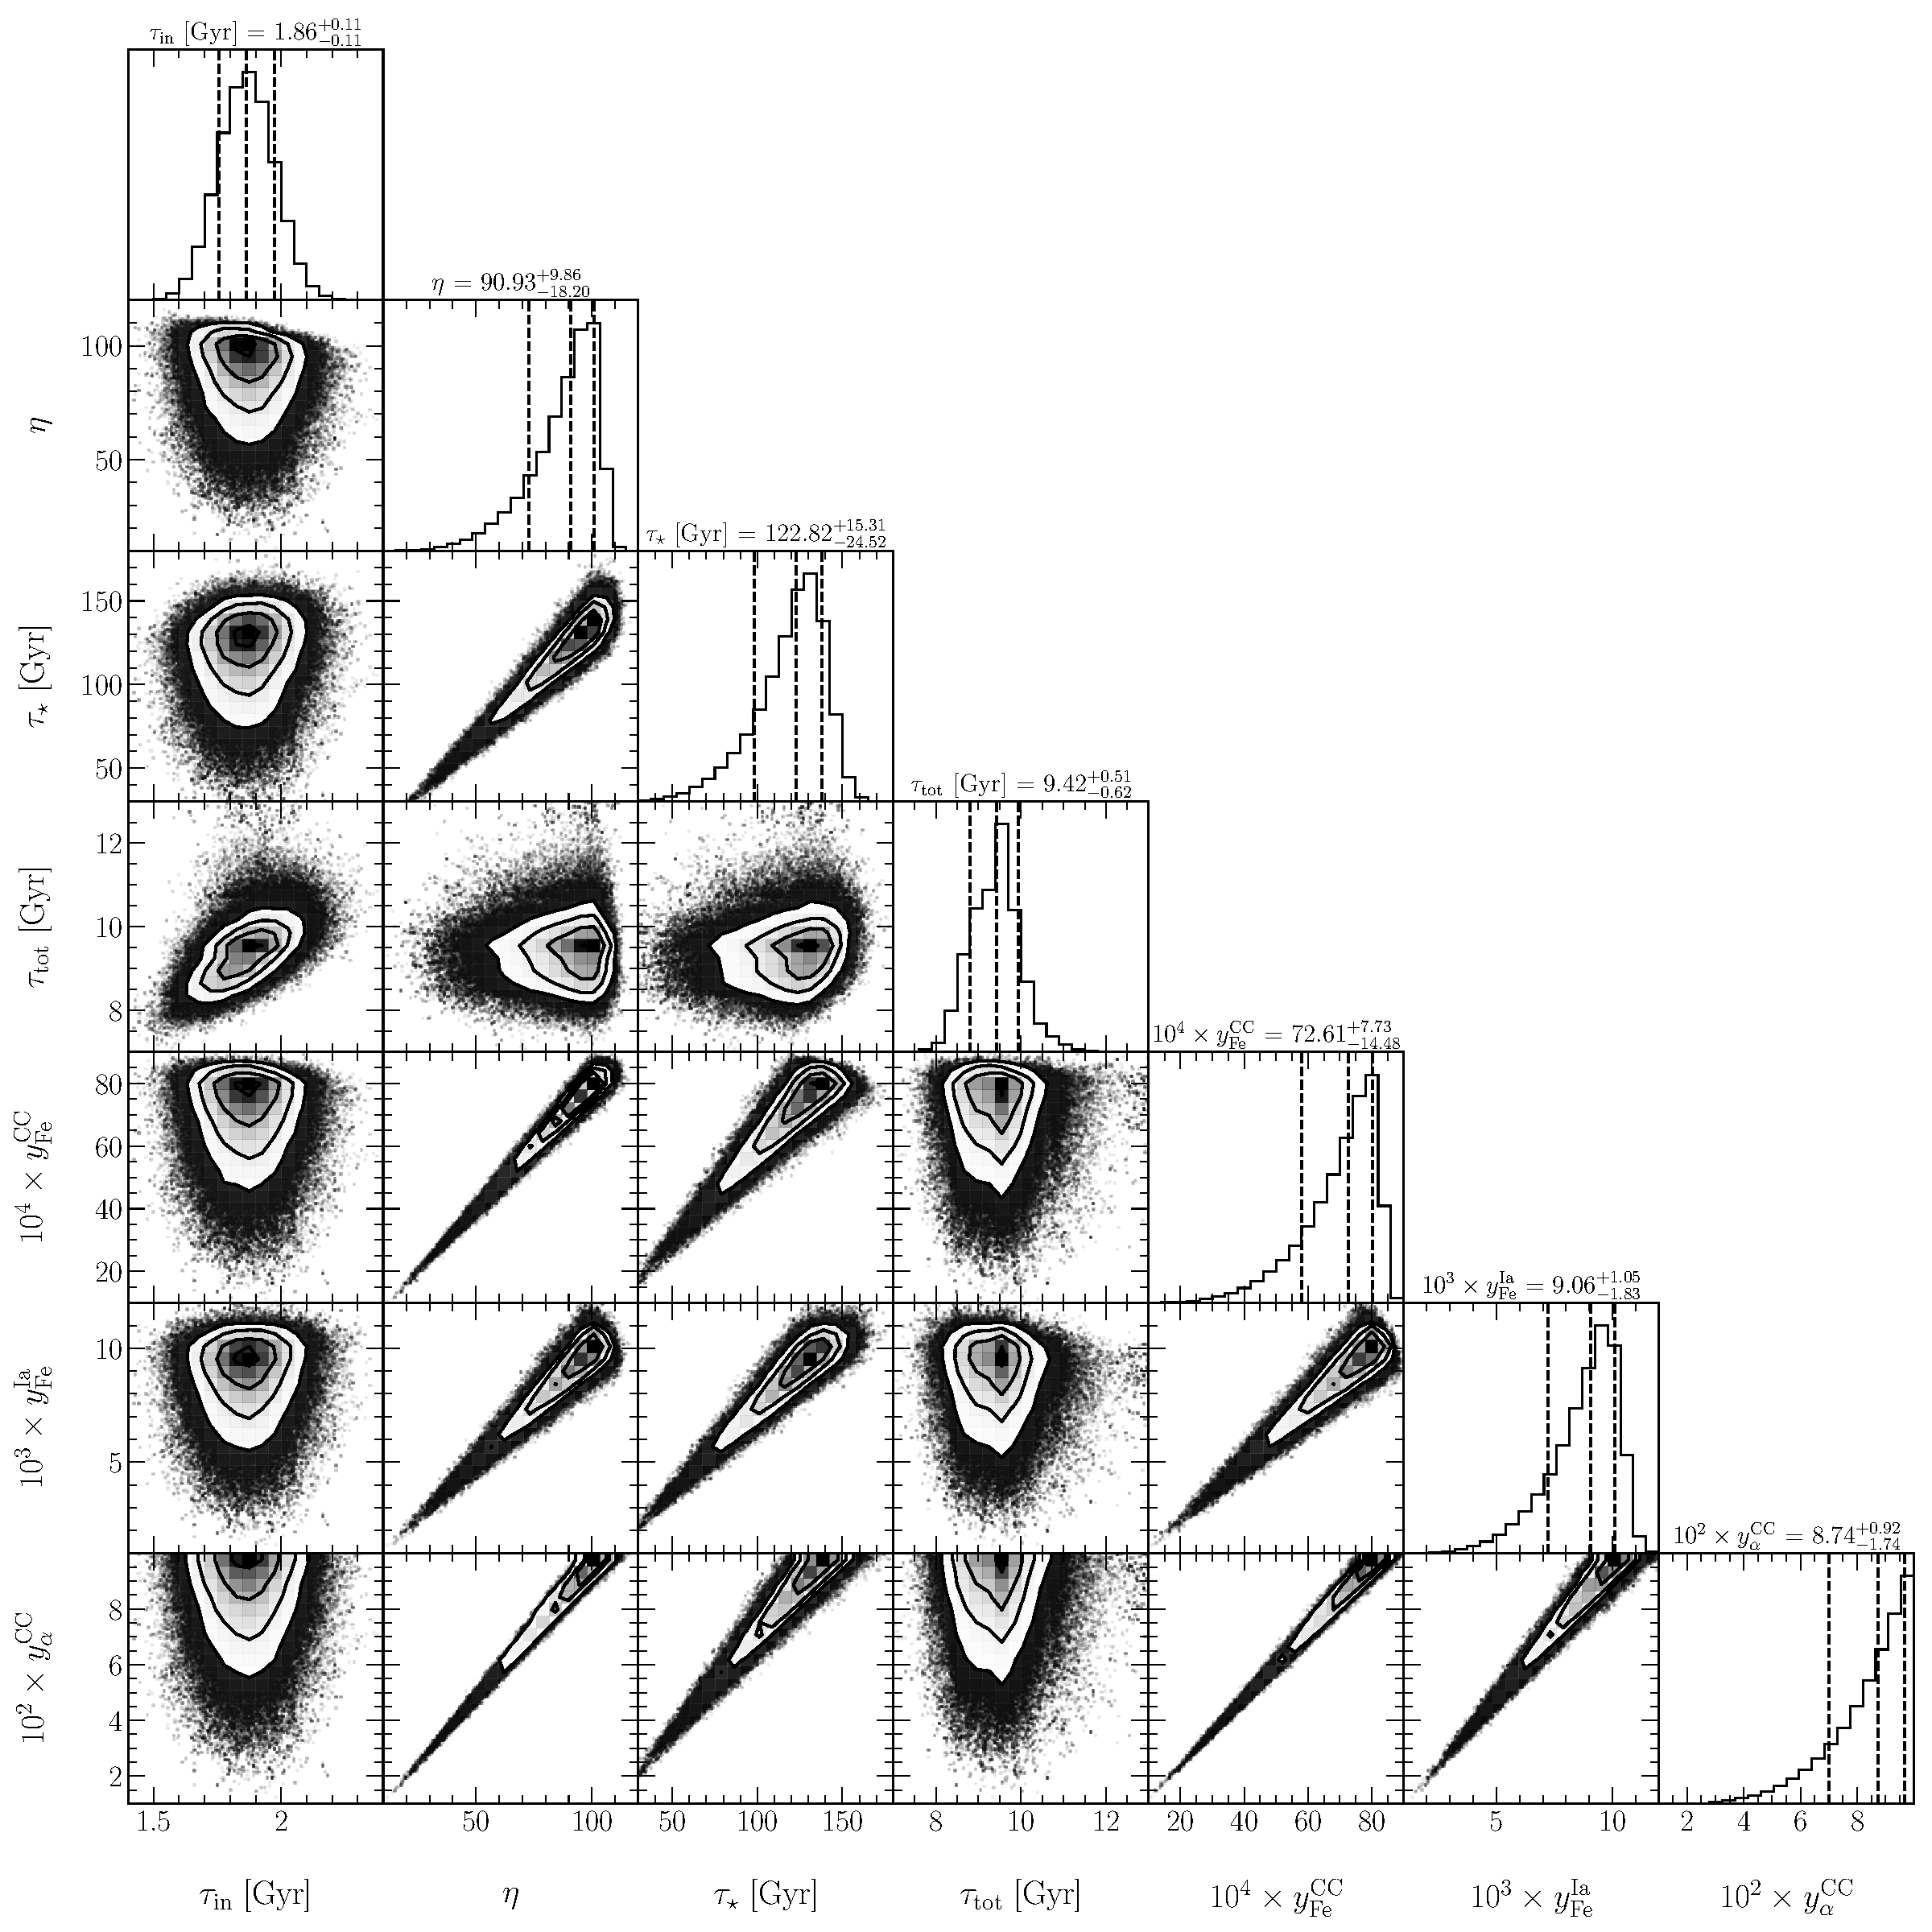
\includegraphics[scale = 0.38]{degeneracy_512k.pdf}
\caption{
The same as Fig.~\ref{fig:fiducial_mock_corner}, but with the alpha element
yield from massive stars~$\yacc$ as an additional free parameter.
Motivated both by theoretical models of O nucleosynthesis in massive stars and
the convenience for scaling parameters up or down, we have adopted
$\yacc = 0.01$ in this paper to set the scale of this degeneracy.
Here we include a prior that enforces~$\yacc < 0.1$, without which the
likelihood distribution extends to arbitrarily high values.
}
\label{fig:degeneracy}
\end{figure*}

Under the instantaneous recycling approximation, early work in GCE demonstrated
that galaxies with ongoing accretion of metal-poor gas reached an equilibrium
metal abundance in which the newly produced metal mass is balanced by losses to
star formation and, if present, outflows (e.g.,~\citealp{Larson1972}, and more
recently~\citealp{Weinberg2017}).
These ``open-box'' models offered a simple solution to the ``closed-box''
models suffering from the so-called ``G-dwarf problem'' whereby the frequency
of super-solar metallicity stars was extremely over-predicted (see the review
in, e.g.,~\citealp{Tinsley1980}).
These results were corroborated by~\citet{Dalcanton2007} who argued that
metal-enriched outflows are the only mechanism that can significantly reduce
effective yields from SNe.
\par
Recent theoretical explorations of SN explosions propose that many massive
stars collapse directly to black holes at the ends of their lives as opposed to
exploding as CCSNe (\citealp{OConnor2011, Pejcha2015, Ertl2016, Sukhbold2016};
see also discussion in~\citealp{Griffith2021}).
This scenario is supported by the observation of a~$\sim$25~\msun~red
supergiant in NGC 6946 (the ``Fireworks Galaxy'') that disappeared from view
after a brief outburst in 2009, indicative of a failed SN
(\citealp*{Gerke2015};~\citealp{Adams2017, Basinger2021}).
These results add to the theoretical uncertainties in stellar evolution and
nuclear reaction networks which significantly impact predicted nucleosynthetic
yields.
% These results challenge the interpretation of~\citet{Dalcanton2007}, instead
% suggesting that SN yields are perhaps~\textit{intrinsically} lower and
% consequently may not require adjusting with metal-enriched outflows to alter
% effective yields.
Observationally, it is feasible to constrain relative but not absolute yields.
For example, the ``two-process model'' (\citealp{Weinberg2019, Weinberg2022};
\citealp*{Griffith2019};~\citealp{Griffith2022}) quantifies the median trends
in abundance ratios relative to Mg along the high- and low-alpha sequences to
disentangle the relative contributions of prompt and delayed nucleosynthetic
sources of various elements.
Yield ratios can also be derived from individual SN remnants as in, e.g.,
\citet*{HollandAshford2020}.
However, these investigations cannot constrain the absolute yields of
individual elements.
\par
In GCE models, there are many parametrizations of outflows.
The publicly available GCE codes~\textsc{FlexCE}~\citep{Andrews2017},
\textsc{OMEGA}~\citep{Cote2017} and~\vice~\citep{Johnson2020} assume the form
of equation~\refp{eq:massloading}, implicitly assuming that massive stars are
the dominant source of energy in outflow-driving winds.
Recently,~\citet{delosReyes2022} modelled the evolution of the Sculptor dwarf
spheroidal by letting the outflow rate be linearly proportional to the the
SN rate~$\dot{N}_\text{II} + \dot{N}_\text{Ia}$.
\citet*{Kobayashi2020} constructed a model for the Milky Way in which
outflows develop in the early phases of the evolution, but die out as the
Galaxy grows.
Based on theoretical models suggesting that the re-accretion timescales of
ejected metals are short ($\sim$100 Myr;~\citealp{Melioli2008, Melioli2009,
Spitoni2008, Spitoni2009}), some authors even neglect outflows entirely when
modelling the Milky Way~\citep[e.g.,][]{Minchev2013, Minchev2014, Minchev2017,
Spitoni2019, Spitoni2021}.
Although these models neglecting outflows are able to reproduce many
observables within the Milky Way disc, this argument is at odds with the
empirical result that multi-phase kiloparsec-scale outflows are ubiquitous
around galaxies of a broad range of stellar masses (see, e.g., the recent
review in~\citealt{Veilleux2020}).
Furthermore, measurements of the deuterium abundance (\citealp{Linsky2006};
\citealp*{Prodanovic2010}) and the~$^3$He/$^4$He ratio~\citep{Balser2018} in
the local ISM indicate near-primordial values.
These results indicate that much of the gas in the Galaxy has not been
processed by stars, further suggesting that ambient ISM is readily swept up in
outflows and replaced by unprocessed baryons through
accretion~\citep{Weinberg2017b, Cooke2022}.
% Although it is possible that much of the deuterium could be depleted onto dust
% grains (\citealp{Romano2006};~\citealp*{Steigman2007}), the same cannot be
% said of~$^3$He or~$^4$He.
\par
Suffice it to say that the community has settled on neither the proper
parametrization nor the importance of mass-loading in GCE models.
As discussed in~\S~\ref{sec:onezone}, the strength of outflows (i.e., the value
of~$\eta$ in this work) is strongly degenerate with the absolute scale of
effective nucleosynthetic yields because they are the primary source and sink
terms in describing enrichment rates (Eq.~\ref{eq:enrichment}).
In this paper, we have applied our fitting method on an assumed scale in which
the oxygen yield from massive stars is fixed at~$\yacc = 0.01$, though if
outflows are to be neglected, the assumption of~$\eta = 0$ fulfills the same
purpose.
While variations in assumptions regarding massive star explodability and the
black hole landscape can lower yields by factors
of~$\sim2 - 3$~\citep{Griffith2021}, values lower by an order of magnitude or
more can be achieved if a significant fraction of SN ejecta is immediately
lost to a hot outflow as proposed by~\citet{Peeples2011}.
Unless star formation is sufficiently slow, this modification is a necessary
for models that assume~$\eta = 0$ as otherwise unphysically high metal
abundances will arise.
There is some observational support for this scenario in that galactic outflows
are observed to be more metal-rich than the ISM of the host galaxy
(\citealp*{Chisholm2018};~\citealp{Cameron2021}), but the metallicities are
not as high as the SN ejecta themselves and cold-phase material is generally
observed in the outflows as well (e.g., in M82,~\citealp{Lopez2020}, and in
NGC 253,~\citealp{Lopez2022}; see also the review in~\citealt{Veilleux2020}).
\par
Motivated by this discourse, we quantify the strength of the yield-outflow
degeneracy by introducing~\yacc~as an additional free parameter in our fit to
our fiducial mock sample described in~\S~\ref{sec:mocks:fiducial}.
We include a prior enforcing~$\yacc < 0.1$; otherwise we find that the MCMC
algorithm allows~$\eta$,~$\tau_\star$ and the SN yields to reach arbitrarily
high values.
Otherwise, we follow the exact same procedure to recover the known evolutionary
parameters of the input model.
Fig.~\ref{fig:degeneracy} shows the resultant posterior distributions.
As expected, there are extremely strong degeneracies in all yields with one
another and with the outflow parameter~$\eta$.
There is an additional degeneracy between the SFE timescale~$\tau_\star$ and
the yields that arises because the position of the ``knee'' in
the~\afe-\feh~plane can be fit with either a high-yield and slow star formation
or a low yield and fast star formation (when we set the overall scale with
$\yacc = 0.01$, we find a degeneracy of the opposite sign; see discussion
in~\S~\ref{sec:mocks:recovered} and in~\citealt{Weinberg2017}).
The strength of these degeneracies is especially striking considering that this
is mock data drawn from an input model with known evolutionary parameters.
In practice, the overall yield scale has factors of~$\sim$$2 - 3$ uncertainty
but not an order of magnitude.
It may therefore be preferable to find best-fit models at a few discrete
values of~\yacc~and understand how other parameters change rather than treat
it as a free parameter.
% We expect the other yields to change in proportion and~$\eta$ to change in
% near proportion, but~$\tau_\star$ may be better constrained than
% Fig.~\ref{fig:degeneracy} suggests.
\par
In detail, this degeneracy arises whenever a parameter influences either the
centroid of the MDF or the position or shape of the evolutionary track in
the~\afe-\feh~diagram.
The infall timescale~$\tau_\text{in}$ and the total duration of star formation
$\tau_\text{tot}$ are unaffected by this degeneracy because they do not
significantly impact these details of the enrichment history (see discussion
in~\S~\ref{sec:mocks:recovered}).
Regardless of the choice of yields and the values of~$\eta$ and~$\tau_\star$,
the shape of the MDF is constrained by a sufficiently large sample, allowing
precise derivations of~$\tau_\text{in}$ and~$\tau_\text{tot}$ with our fitting
method.
Determining the duration of star formation in this manner may open a new
pathway for constraining the early epochs of star formation in both intact
and disrupted dwarf galaxies as well as deriving quenching times for the
now-quiescent systems (see discussion in~\S~\ref{sec:mocks:variations}).

\end{document}
